\documentclass[aspectratio=169,11pt]{beamer}
\usepackage[T1]{fontenc}
\usepackage[utf8]{inputenc}
\usepackage{lmodern,amsmath,amssymb,graphicx,tikz}
\usetikzlibrary{arrows.meta,calc}
\usetheme{default}
\usefonttheme{serif}
\setbeamercolor{normal text}{fg=black,bg=white}
\setbeamercolor{structure}{fg=black}
\setbeamercolor{frametitle}{fg=black}
\setbeamercolor{title}{fg=black}
\setbeamertemplate{navigation symbols}{}
\setbeamertemplate{footline}[frame number]
\setbeamertemplate{itemize items}[circle]
\setbeamersize{text margin left=8mm,text margin right=8mm}
\setlength{\parskip}{5pt}
\newcommand{\cO}{\mathcal O}
\newcommand{\cI}{\mathcal I}
\newcommand{\cA}{\mathcal A}
\newcommand{\db}{\bar\partial}
\newcommand{\C}{\mathbb C}
\newcommand{\Pj}{\mathbb P}
\newcommand{\norm}[1]{\lVert#1\rVert}
\newcommand{\src}[1]{\par\vfill{\scriptsize #1\par}}
\author{Daniel Gonz\'alez Casanova Azuela}

\title{Kodaira embedding theorem (Part 2)}
\subtitle{From solving \(\bar\partial\) to projective coordinates}
\date{Hodge theory, IMPA \quad 16 November 2026}
\begin{document}
\begin{frame}\titlepage\end{frame}

\begin{frame}{The goal}
Let \(X\) be compact complex and \(L\) a positive holomorphic line bundle.
\par\bigskip
We want one power \(A=L^N\) whose global sections:
\begin{enumerate}
\setlength{\itemsep}{12pt}
\item have no common zero;
\item separate distinct points;
\item separate tangent directions.
\end{enumerate}
\par\bigskip
These give an everywhere-defined injective holomorphic immersion into projective space.
\end{frame}

\begin{frame}{Nadel: the vanishing we need}
On compact Kähler \((X,\omega)\), if a singular metric \(h\) on \(B\) satisfies \(i\Theta_h\ge\varepsilon\omega\), \(\varepsilon>0\), then
\[
\boxed{H^1(X,K_X\otimes B\otimes\cI(h))=0.}
\]
Take \(B=L^N\otimes K_X^{-1}\). Then \(K_X\otimes B=L^N=A\), so
\[
\boxed{H^1(X,A\otimes\cI(h))=0.}
\]
We must choose the metric so that its ideal imposes the data we want.
\end{frame}

\begin{frame}{Reminder: the multiplier ideal}
\label{fr:mi-def}
\textbf{Setting.} \(h\) is a singular metric on \(B\). Near a point \(x\), choose a holomorphic frame \(e\) of \(B\) and write \(|e|_h^2=e^{-2\varphi}\), with \(\varphi\) psh.
\par\medskip
A holomorphic section of \(B\) near \(x\) is \(s=fe\), with \(f\) a holomorphic function. Its length is
\[
|s|_h^2=|f|^2e^{-2\varphi}.
\]
\textbf{Question.} Is \(|s|_h^2\) integrable near \(x\)?
\par\medskip
\textbf{Definition.} The multiplier ideal collects the \(f\) for which the answer is yes:
\[
\boxed{\cI(h)_x=\Bigl\{f\in\cO_{X,x}:\ \int_U|f|^2e^{-2\varphi}\,dV<\infty\ \text{for some neighbourhood } U \text{ of } x\Bigr\}.}
\]
\textbf{So} \(B\otimes\cI(h)\) is the sheaf of holomorphic sections of \(B\) that are locally square-integrable for \(h\).
\src{Lecture 23, slide 41. M.~Verbitsky, \emph{Hodge theory}, lecture 23 (2025), slide 2.}
\end{frame}

\begin{frame}{Reminder: what the multiplier ideal measures}
\label{fr:mi-measures}
The question was: is \(|f|^2e^{-2\varphi}\) integrable near \(x\)? The answer depends on \(\varphi\) near \(x\).
\par\bigskip
\begin{itemize}
\setlength{\itemsep}{12pt}
\item \textbf{If \(\varphi\) is bounded near \(x\),} the answer is always yes:
\[
\cI(h)_x=\cO_{X,x}.
\]
\item \textbf{If \(\varphi(x)=-\infty\),} the weight \(e^{-2\varphi}\) is infinite at \(x\). The answer is yes only if \(f\) vanishes at \(x\) fast enough.
\end{itemize}
\par\bigskip
\textbf{So} the ideal sees only the points where \(\varphi=-\infty\), and at such a point it records how fast \(f\) must vanish.
\par\bigskip
We recall the one example where we computed this when we need it (slide \hyperlink{fr:mi-logpole}{\pageref{fr:mi-logpole}}).
\src{Lecture 23, slide 41. M.~Verbitsky, \emph{Hodge theory}, lecture 23 (2025), slide 2.}
\end{frame}

\begin{frame}{The proof of Nadel uses \(L^2\) forms: the sheaves \(\mathcal L^{n,q}\)}
\label{fr:l2-def}
In the proof of Kodaira vanishing the forms were smooth. In the proof of Nadel vanishing the metric \(h\) is singular, and the forms are square-integrable.
\par\medskip
\textbf{Reminder} (lecture 23, slide 55). \(\mathcal L^{n,q}\) is the sheaf of \(B\)-valued \((n,q)\)-forms \(u\) with measurable coefficients such that
\begin{enumerate}
\item \(|u|_h^2\) is locally integrable;
\item \(|\db u|_h^2\) is locally integrable.
\end{enumerate}
\par\medskip
\textbf{Plan.}
\begin{itemize}
\item What conditions 1 and 2 mean (slides \hyperlink{fr:l2-first}{\pageref{fr:l2-first}} to \hyperlink{fr:l2-second-gives}{\pageref{fr:l2-second-gives}}).
\item Smooth forms and \(L^2\) forms side by side (slide \hyperlink{fr:smooth-vs-l2}{\pageref{fr:smooth-vs-l2}}).
\item In degree \(0\) the kernel of \(\db\) is \(K_X\otimes B\otimes\cI(h)\) (slide \hyperlink{fr:l2-kernel}{\pageref{fr:l2-kernel}}).
\end{itemize}
\end{frame}

\begin{frame}{Condition 1: \(|u|_h^2\) is locally integrable}
\label{fr:l2-first}
In a holomorphic frame \(e\) of \(B\), with \(|e|_h^2=e^{-2\varphi}\) and \(\varphi\) psh, a form \(u=v\otimes e\) has
\[
|u|_h^2=|v|^2e^{-2\varphi}.
\]
So condition 1 says: \(|v|^2e^{-2\varphi}\) is locally integrable.
\par\medskip
The definition does not need \(\varphi\) psh. \textbf{What psh adds:}
\begin{itemize}
\item \(\varphi\) is locally integrable, by the mean value inequality (lecture 23, slide 35). So \(\varphi>-\infty\) almost everywhere, and the weight \(e^{-2\varphi}\) is finite almost everywhere.
\item \(\varphi\) is locally bounded above, \(\varphi\le M\), by upper semicontinuity (lecture 23, slide 35). So \(e^{-2\varphi}\ge e^{-2M}\) and
\[
\int_U|v|^2\,dV\le e^{2M}\int_U|v|^2e^{-2\varphi}\,dV .
\]
Square-integrable for \(h\) implies square-integrable in the usual sense. So \(u\) is a distribution, and \(\db u\) makes sense.
\end{itemize}
\end{frame}

\begin{frame}{Condition 1: a warning, and what it is for}
\label{fr:l2-first-gives}
\textbf{Warning.} The converse fails: square-integrable in the usual sense does not imply square-integrable for \(h\).
\par\smallskip
\textbf{Example.} Take \(\varphi=a\log|z|\) on \(\C^n\) and the form with constant coefficient \(v=1\). It is smooth and square-integrable in the usual sense. But
\[
|v|^2e^{-2\varphi}=|z|^{-2a}
\]
is integrable near \(0\) only if \(a<n\). So for \(a\ge n\) this form fails condition 1.
\par\smallskip
This is the rule \(k>a-n\) of slide \hyperlink{fr:mi-logpole}{\pageref{fr:mi-logpole}} for \(k=0\). A coefficient that vanishes at \(0\) to order \(k>a-n\) still satisfies condition 1.
\par\medskip
\textbf{What it is for.} On compact \(X\), the global forms with \(\int_X|u|_h^2\,dV<\infty\) form a Hilbert space. The Hilbert-space lemma (slide \hyperlink{fr:hilbert-lemma}{\pageref{fr:hilbert-lemma}}) works there.
\end{frame}

\begin{frame}{Condition 2: \(|\db u|_h^2\) is locally integrable}
\label{fr:l2-second}
By condition 1, \(u\) is square-integrable in the usual sense (slide \hyperlink{fr:l2-first}{\pageref{fr:l2-first}}). So \(\db u\) exists as a distribution: it is defined by integrating \(u\) against derivatives of smooth compactly supported forms.
\par\medskip
\textbf{But \(\db u\) need not be a function.} On \(\C\) let \(u=1\) for \(\operatorname{Re}z>0\) and \(u=0\) otherwise. Then \(u\) is locally square-integrable, and
\[
\frac{\partial u}{\partial\bar z}=\frac12\,\frac{\partial u}{\partial x}
\]
is half the delta measure on the line \(\operatorname{Re}z=0\). It is not a square-integrable function.
\par\medskip
Condition 2 asks that \(\db u\) is again a form satisfying condition 1.
\src{\textcolor{red}{I did not verify this slide.}}
\end{frame}

\begin{frame}{Condition 2: what it is for}
\label{fr:l2-second-gives}
\textbf{It makes \(\db\) a map of sheaves}
\[
\db:\mathcal L^{n,q}\to\mathcal L^{n,q+1}.
\]
Indeed, for \(u\in\mathcal L^{n,q}\) the form \(\db u\) satisfies condition 1 by assumption, and condition 2 because \(\db(\db u)=0\).
\par\medskip
So the \(\mathcal L^{n,q}\) form a complex, like the smooth forms in the Dolbeault complex.
\par\medskip
\textbf{In operator language.} Condition 1 says \(u\) is in the Hilbert space. Condition 2 says \(u\) is in the domain of \(\db\).
\par\medskip
\textbf{Why ``locally''.} A sheaf is defined by conditions on small open sets. On compact \(X\), locally integrable is the same as integrable.
\end{frame}

\begin{frame}{Smooth forms and \(L^2\) forms side by side}
\label{fr:smooth-vs-l2}
\begin{center}
\renewcommand{\arraystretch}{1.0}
\begin{tabular}{ll}
\hline
\(\mathcal A^{n,q}(B)\) & smooth coefficients\\
\(\mathcal L^{n,q}\) & measurable coefficients, with conditions 1 and 2\\
\hline
\(\Omega^n_X\otimes B\) & holomorphic coefficients (\(q=0\) only)\\
\(\Omega^n_X\otimes B\otimes\cI(h)\) & holomorphic coefficients, with condition 1 (\(q=0\) only)\\
\hline
\(\cI(h)\subset\cO_X\) & holomorphic functions \(f\) with \(|f|^2e^{-2\varphi}\) locally integrable\\
\hline
\end{tabular}
\end{center}
\vspace{-6pt}
In each, the kernel of the first \(\db\) is the sheaf of holomorphic sections:
\[
\begin{array}{l}
\ker\bigl(\db:\mathcal A^{n,0}(B)\to\mathcal A^{n,1}(B)\bigr)=\Omega^n_X\otimes B\\
\ker\bigl(\db:\mathcal L^{n,0}\to\mathcal L^{n,1}\bigr)=\Omega^n_X\otimes B\otimes\cI(h)
\end{array}
\]
\par\vspace{-8pt}\noindent
\textbf{Why \(\Omega^n_X\) appears.} For \(u=f\,dz_1\wedge\cdots\wedge dz_n\otimes e\), \(\db u=0\) makes \(f\) holomorphic: \(\db f\) contains only the \(d\bar z_k\), linearly independent of the \(dz_j\).
\par\vspace{1pt}
\textbf{Why \(\Omega^n_X\otimes B\otimes\cI(h)\) appears.} \(f\) is holomorphic by being in \(\ker\db\) (regularity, not proved), and in \(\cI(h)\) because \(|f|^2e^{-2\varphi}\) was taken locally integrable.
\par\vspace{1pt}
\textbf{Why \(q=0\) only.} For \(q>0\) we just get \(\mathcal A^{n,q}(B)\) and \(\mathcal L^{n,q}\): forms of degree \(n+q>n\), and a holomorphic form has degree at most \(n\).
\end{frame}

\begin{frame}{The two resolutions}
\label{fr:l2-kernel}
The holomorphic sheaves appear only at the start. Both sequences are exact (smooth: Dolbeault--Grothendieck lemma; \(L^2\): not proved):
\[
\begin{array}{l}
0\to\Omega^n_X\otimes B\to\mathcal A^{n,0}(B)\xrightarrow{\db}\mathcal A^{n,1}(B)\xrightarrow{\db}\cdots\\[3pt]
0\to\Omega^n_X\otimes B\otimes\cI(h)\to\mathcal L^{n,0}\xrightarrow{\db}\mathcal L^{n,1}\xrightarrow{\db}\cdots
\end{array}
\]
The sheaves \(\mathcal A^{n,q}(B)\), \(\mathcal L^{n,q}\) are fine, so on global sections, in degree \(q\),
\[
\begin{array}{ll}
H^q(X,\Omega^n_X\otimes B)=\ker\db/\operatorname{im}\db&\text{in }\mathcal A^{n,q}(B)\quad\text{(Dolbeault)}\\[3pt]
H^q(X,\Omega^n_X\otimes B\otimes\cI(h))=\ker\db/\operatorname{im}\db&\text{in }\mathcal L^{n,q}
\end{array}
\]
\textbf{Nadel:} show the second group is trivial for \(q=1\), by letting \(\db f=0\) with \(f\) a global section of \(\mathcal L^{n,1}\), and finding a global section \(u\) of \(\mathcal L^{n,0}\) with \(\db u=f\).
\par\smallskip
Note that \(\db u=f\) is an equation on forms. Locally, for \(u=v\,dz_1\wedge\cdots\wedge dz_n\otimes e\) and \(f=\sum_jg_j\,d\bar z_j\wedge dz_1\wedge\cdots\wedge dz_n\otimes e\), it is a system: one unknown function \(v\) and \(n\) equations \(\partial v/\partial\bar z_j=g_j\).
\end{frame}

\begin{frame}{Why does \(K_X\) appear?}
\label{fr:why-nq}
\label{fr:KX-summary}
\begin{center}
\fbox{\parbox{0.92\textwidth}{\textbf{Because we need a pairing.} To compute cohomology we pair forms by integrating over \(X\). A \((0,q)\)-form can only be integrated against a form of the complementary type \((n,n-q)\), and such a form contains \(dz_1\wedge\cdots\wedge dz_n\): a section of \(K_X\).}}
\end{center}
\begin{itemize}
\setlength{\itemsep}{12pt}
\item \textbf{It is not because of the resolution.} For every \(p\), the \((p,q)\)-forms with values in \(B\) resolve \(\Omega^p_X\otimes B\). With \(p=0\) we resolve \(\cO_X\otimes B\), and there is no \(K_X\).
\item \textbf{The pairing is how we compute.} Serre duality describes the dual of a cohomology group with it. Kodaira and Nadel vanishing are the case where the group is zero.
\item \textbf{Calabi--Yau manifolds:} \(K_X\) is trivial, so \(\Omega^n_X\cong\cO_X\) and the difference disappears.
\end{itemize}
\par\medskip
Details: the next slide.
\end{frame}


\begin{frame}{How the pairing computes cohomology: the Hilbert-space lemma}
\label{fr:linalg-adjoint}
\label{fr:hilbert-lemma}
\(T:V\to W\) is linear, \(V\) and \(W\) have inner products (the pairing), and \(T^*:W\to V\) is the adjoint: \(\langle Tu,v\rangle=\langle u,T^*v\rangle\).
\par\medskip
\textbf{1. The vectors orthogonal to the image are \(\ker T^*\).}
\[
v\perp\operatorname{im}T\iff\langle Tu,v\rangle=0\ \text{for all }u\iff\langle u,T^*v\rangle=0\ \text{for all }u\iff T^*v=0 .
\]
\textbf{2. In finite dimensions} the image is \((\ker T^*)^\perp\): \(\ Tu=f\) is solvable exactly when \(f\perp\ker T^*\).
\par\medskip
\textbf{3. In Hilbert spaces: the lemma.} For closed densely defined operators \(H_1\xrightarrow{T}H_2\xrightarrow{S}H_3\) with \(\operatorname{im}T\subset\ker S\), suppose
\[
C\|v\|^2\le\|T^*v\|^2+\|Sv\|^2,\qquad C>0,
\]
for all \(v\) in \(\operatorname{Dom}T^*\cap\operatorname{Dom}S\). Then
\[
\boxed{Sf=0\quad\Longrightarrow\quad Tu=f\text{ for some }u.}
\]
\textbf{For Nadel:} slide \hyperlink{fr:nadel-estimate}{\pageref{fr:nadel-estimate}} gives the three spaces and the estimate, with \(C=\varepsilon\).
\end{frame}


\begin{frame}{The essential idea of the Hilbert-space proof}
\label{fr:hilbert-idea}
\textbf{Given:} \(f\) with \(Sf=0\). \textbf{Unknown:} \(u\). \textbf{Wanted:} \(Tu=f\).
\par\medskip
\textbf{1. Rewrite the goal with the pairing.} \(Tu=f\) means \(\langle Tu,v\rangle=\langle f,v\rangle\) for all \(v\), that is
\[
\langle u,T^*v\rangle=\langle f,v\rangle\quad\text{for all } v .\tag{$*$}
\]

\textbf{2. Riesz representation theorem.} For every \textbf{bounded} linear functional \(\ell\) on a Hilbert space \(H\) there is a unique \(u\in H\) with \(\ell(w)=\langle w,u\rangle\) for all \(w\), and \(\|u\|=\|\ell\|\). Bounded means: \(|\ell(w)|\le M\|w\|\) for some \(M\).
\par\medskip
\textbf{3. Our functional} is \(\ell(T^*v)=\langle f,v\rangle\), on the vectors \(w=T^*v\). For it, ``bounded'' reads
\[
\boxed{|\langle f,v\rangle|\le M\,\|T^*v\| ,\qquad M=C^{-1/2}\|f\| .}
\]
This is the key inequality (next slide; it uses \(C>0\)). Then Riesz gives \(u\) satisfying \((*)\), so \(Tu=f\).
\end{frame}


\begin{frame}{The key inequality: where the constant \(C\) is used}
\label{fr:hilbert-key}
\textbf{Claim.} If \(Sf=0\), then \(\ |\langle f,v\rangle|\le C^{-1/2}\,\|f\|\,\|T^*v\|\ \) for every \(v\).
\par\medskip
\textbf{Split} \(v=v_1+v_2\), with \(v_1\in\ker S\) and \(v_2\perp\ker S\).
\begin{enumerate}
\setlength{\itemsep}{6pt}
\item \(\langle f,v_2\rangle=0\), because \(f\in\ker S\) and \(v_2\perp\ker S\). So \(\langle f,v\rangle=\langle f,v_1\rangle\).
\item \(T^*v_2=0\), because \(v_2\perp\ker S\supset\operatorname{im}T\), and the vectors orthogonal to \(\operatorname{im}T\) are \(\ker T^*\) (slide \hyperlink{fr:linalg-adjoint}{\pageref{fr:linalg-adjoint}}). So \(T^*v=T^*v_1\).
\item The estimate \(C\|v_1\|^2\le\|T^*v_1\|^2+\|Sv_1\|^2\), with \(Sv_1=0\), gives
\[
\|v_1\|\le C^{-1/2}\,\|T^*v_1\|=C^{-1/2}\,\|T^*v\| .
\]
\end{enumerate}
\textbf{Together} (Cauchy--Schwarz):
\[
|\langle f,v\rangle|=|\langle f,v_1\rangle|\le\|f\|\,\|v_1\|\le C^{-1/2}\,\|f\|\,\|T^*v\| .
\]
If \(C\) were \(0\) there would be no bound, and no \(u\).
\src{\textcolor{red}{I did not verify this slide.}}
\end{frame}



\begin{frame}{The estimate for Nadel}
\label{fr:nadel-estimate}
\textbf{The lemma (slide \hyperlink{fr:hilbert-lemma}{\pageref{fr:hilbert-lemma}}) needs:}\quad
\(H_1\xrightarrow{T}H_2\xrightarrow{S}H_3\)\quad and\quad \(C\norm{v}^2\le\norm{T^*v}^2+\norm{Sv}^2\).
\par\smallskip
\textbf{For Nadel.} \(H_1,H_2,H_3\) are the global \(L^2\) forms of type \((n,0),(n,1),(n,2)\) with values in \(B\), and \(T=S=\db\), \(T^*=\db^*\).
\par\smallskip
\textbf{Bochner--Kodaira--Nakano} (lecture 23, slide 19):
\[
\boxed{\Delta_{\db}=\Delta_{\partial}+[\,i\Theta_h\wedge,\Lambda\,].}
\]
Use \(\Delta_{\db}=\db\db^*+\db^*\db\), \(\Delta_{\partial}=\partial\partial^*+\partial^*\partial\), pair with \(v\), use adjointness, integrate:
\[
\norm{\db v}^2+\norm{\db^*v}^2
=\underbrace{\norm{\partial v}^2+\norm{\partial^*v}^2}_{\ge0}
+\underbrace{\int_X\big\langle[\,i\Theta_h\wedge,\Lambda\,]v,v\big\rangle\,dV}_{\ge\,\varepsilon\norm{v}^2}.
\]
The second bound is where \(i\Theta_h\ge\varepsilon\omega\) is used. So \(\ \boxed{\norm{\db^*v}^2+\norm{\db v}^2\ge\varepsilon\norm{v}^2}\ \) and \(C=\varepsilon\).
\par
That this holds for \(L^2\) forms and a singular \(h\) is an analytic input (not proved).
\end{frame}

\begin{frame}{Nadel is done}
\label{fr:nadel-done}
\begin{center}
\(\boxed{i\Theta_h\ge\varepsilon\omega\quad\Longrightarrow\quad H^1(X,K_X\otimes B\otimes\cI(h))=0}\)
\end{center}
\par\medskip
What we did:
\begin{enumerate}
\setlength{\itemsep}{6pt}
\item \(H^1\) is \(\ker\db/\operatorname{im}\db\) on global \(L^2\) forms (slide \hyperlink{fr:l2-kernel}{\pageref{fr:l2-kernel}}).
\item So \(H^1=0\) becomes: solve \(\db u=f\) for every \(f\) with \(\db f=0\).
\item Curvature \(i\Theta_h\ge\varepsilon\omega\) gives a solution: through the estimate (slide \hyperlink{fr:nadel-estimate}{\pageref{fr:nadel-estimate}}) and the Hilbert-space lemma (slide \hyperlink{fr:hilbert-lemma}{\pageref{fr:hilbert-lemma}}).
\end{enumerate}
\par\medskip
From now on Nadel is a tool. We use it to build sections of \(A=L^N\) and prove the Kodaira embedding theorem.
\end{frame}

\begin{frame}{The map \(\Phi\) of Kodaira embedding}
\label{fr:need}
With \(A=L^N\), send a point \(x\) to ``evaluate sections at \(x\)'':
\[
\boxed{\Phi:X\to\Pj\bigl(H^0(X,A)^*\bigr),\qquad \Phi(x)=[\operatorname{ev}_x],\qquad \operatorname{ev}_x(s)=s(x).}
\]
In a basis \(s_0,\ldots,s_M\) of \(H^0(X,A)\), with dual basis \(s_0^*,\ldots,s_M^*\):
\[
\begin{array}{r@{\,=\,}l}
\operatorname{ev}_x & s_0(x)\,s_0^*+s_1(x)\,s_1^*+\cdots+s_M(x)\,s_M^*\\[3pt]
s & s_0^*(s)\,s_0+s_1^*(s)\,s_1+\cdots+s_M^*(s)\,s_M
\end{array}
\]
The first line gives the coordinates of \(\Phi(x)\), the second those of \(s\):
\[
\Phi(x)=[\,s_0(x):s_1(x):\cdots:s_M(x)\,]\in\Pj^M,\qquad s=(s_0^*(s),s_1^*(s),\ldots,s_M^*(s)).
\]
\end{frame}




\begin{frame}{What do we need for a holomorphic embedding?}
\label{fr:goal-sections}
We want \(\Phi\) to be a holomorphic embedding. What do we need?
\begin{enumerate}
\setlength{\itemsep}{10pt}
\item \textbf{\(\Phi\) well defined.} At every \(x\), not all coordinates \(s_i(x)\) are zero: some section \(s\) has \(s(x)\ne0\). This is ``\textbf{no common zero}''. Then \(\Phi\) is holomorphic: where \(s_j\ne0\), its coordinates are the quotients \(s_i/s_j\), which are holomorphic functions.
\item \textbf{\(\Phi\) injective.}
\item \textbf{\(\Phi\) an immersion:} \(d\Phi_x\) is injective at every \(x\).
\end{enumerate}
\par\medskip
\(X\) is compact, so an injective immersion is closed, hence an embedding.
\end{frame}


\begin{frame}{Injectivity: separating points}
\label{fr:prov-injective}
\textbf{We want injectivity:} \(\Phi(x)\ne\Phi(y)\) whenever \(x\ne y\).
\par\bigskip
\[
\boxed{\Phi(x)=\Phi(y)\iff s(y)=\lambda\,s(x)\text{ for every section }s,\ \lambda\in\C.}
\]
A section \(s\) with \(s(x)=0\) and \(s(y)\ne0\) makes this impossible: \(s(y)=\lambda\,s(x)=0\).
\par\bigskip
\textbf{So we want the ``separates points'' condition:}
\[
\boxed{\text{for every } x\ne y \text{ there is a global section } s \text{ with } s(x)=0 \text{ and } s(y)\ne0.}
\]
The converse is also true: if \(\Phi\) is injective, such sections exist. We do not need it.
\end{frame}




\begin{frame}{Immersion: separating tangent directions}
\label{fr:immersion}
\textbf{We want an immersion:} \(d\Phi_x(v)\ne0\) for every \(x\) and every tangent \(v\ne0\).
\[
\boxed{d\Phi_x(v)=0\iff\text{there is a constant }\mu\text{ with } ds(v)=\mu\,s(x)\text{ for every section }s.}
\]
Here \(ds(v)\) is the derivative along \(v\), at \(x\), of the coefficient of \(s\) in a local frame of \(A\).
\par\smallskip
\textbf{1.} If \(s_0(x)\ne0\), \(\Phi=(s_1/s_0,\ldots,s_M/s_0)\) near \(x\): \(d\Phi_x(v)=0\) means all \(d(s_i/s_0)(v)=0\).
\par
\textbf{2. Quotient rule.}
\[
d\Bigl(\frac{s_i}{s_0}\Bigr)(v)=\frac{ds_i(v)\,s_0(x)-s_i(x)\,ds_0(v)}{s_0(x)^2}=0
\iff ds_i(v)=\mu\,s_i(x),\quad \mu=\frac{ds_0(v)}{s_0(x)} .
\]
The same \(\mu\) for every \(i\), hence, by linearity, for every section \(s=\sum c_is_i\).
\par
\textbf{3. A witness:} \(s\) with \(s(x)=0\), \(ds(v)\ne0\). Then \(ds(v)=\mu\,s(x)=0\) is impossible.
\par
\textbf{So we want the ``separates tangent directions'' condition:}
\[
\boxed{\text{for every } x \text{ and } v\ne0 \text{ there is a global section } s \text{ with } s(x)=0 \text{ and } ds(v)\ne0.}
\]
\end{frame}



\begin{frame}{How algebraic geometry gives the three conditions}
\label{fr:plan}
\label{fr:ideals-data}
Each condition asks for a section of \(A=L^N\) with chosen data at one or two points:
\begin{center}
\renewcommand{\arraystretch}{1.0}
\begin{tabular}{@{}llll@{}}
\hline
condition & we choose & on & ideal \(I\)\\
\hline
no common zero & \(s(x)\ne0\) & the point \(x\) & \(\mathfrak m_x\)\\
separates points & \(s(x)=0\), \(s(y)\ne0\) & two points \(x\ne y\) & \(\mathfrak m_x\cap\mathfrak m_y\)\\
separates tangents & \(s(x)=0\), \(ds(v)\ne0\) & the fat point \(x\) & \(\mathfrak m_x^2\)\\
\hline
\end{tabular}
\end{center}
\textbf{The exact sequence} \(\ 0\to A\otimes I\to A\to A\otimes\cO_X/I\to0\ \) gives
\[
H^0(X,A)\xrightarrow{\ \text{restrict}\ }H^0(X,A\otimes\cO_X/I)\longrightarrow H^1(X,A\otimes I).
\]
\[
\boxed{H^1(X,A\otimes I)=0\quad\Longrightarrow\quad\text{restrict is surjective.}}
\]
\textbf{Why this gives ``no common zero''}, \(I=\mathfrak m_x\). The sheaf \(\cO_X/\mathfrak m_x\) is \(\C\) at \(x\) and zero elsewhere. So the middle space is the fibre \(A_x\), and restrict is \(s\mapsto s(x)\). Surjective: every vector of \(A_x\) is \(s(x)\) for some global \(s\). Choose a nonzero one: \(s(x)\ne0\).
\end{frame}

\begin{frame}{Surjectivity gives ``separates points''}
\label{fr:surj-points}
Take \(I=\mathfrak m_x\cap\mathfrak m_y\) with \(x\ne y\): the functions vanishing at \(x\) and at \(y\).
\par\medskip
\textbf{1. The quotient.} Away from \(x\) and \(y\) the ideal is all of \(\cO_X\), so the quotient is zero there. Near \(x\) it is \(\mathfrak m_x\), near \(y\) it is \(\mathfrak m_y\). So \(\cO_X/I\) is \(\C\) at \(x\), \(\C\) at \(y\), and zero elsewhere.
\par\medskip
\textbf{2. The data.}
\[
H^0(X,A\otimes\cO_X/I)=A_x\oplus A_y,\qquad\text{restrict}(s)=\bigl(s(x),s(y)\bigr).
\]
\textbf{3. Surjective} means: every pair (a vector of \(A_x\), a vector of \(A_y\)) is \(\bigl(s(x),s(y)\bigr)\) for some global section \(s\).
\par\medskip
\textbf{4. Choose the pair} \((0,\text{nonzero})\):
\[
\boxed{\text{a global section } s \text{ with } s(x)=0 \text{ and } s(y)\ne0.}
\]
This is ``separates points'' (slide \hyperlink{fr:prov-injective}{\pageref{fr:prov-injective}}).
\end{frame}

\begin{frame}{The ideal \(\mathfrak m_x^2\) and what its quotient remembers}
\label{fr:m2}
\textbf{The third ideal} (lecture 23, slide 53):
\[
\boxed{\mathfrak m_x^2=\{u:\ u(x)=0\text{ and all first derivatives of }u\text{ vanish at }x\}.}
\]
\begin{itemize}
\item \(\subset\): Leibniz. If \(f(x)=g(x)=0\), then \(\partial_i(fg)(x)=\partial_if(x)\,g(x)+f(x)\,\partial_ig(x)=0\).
\item \(\supset\): since \(u(x)=0\), every monomial of its power series contains some \(z_i\). Pull out one variable from each: \(u=z_1g_1+\cdots+z_ng_n\), with \(g_i(x)=\frac{\partial u}{\partial z_i}(x)=0\). So \(u\) is a sum of products of two elements of \(\mathfrak m_x\).
\end{itemize}
\textbf{The class modulo \(\mathfrak m_x^2\).} Two germs \(u,u'\) have the same class when \(u-u'\in\mathfrak m_x^2\):
\[
(u-u')(x)=0\quad\text{and}\quad\partial_i(u-u')(x)=0\ \text{ for all } i,
\]
that is,
\[
u(x)=u'(x)\quad\text{and}\quad\frac{\partial u}{\partial z_i}(x)=\frac{\partial u'}{\partial z_i}(x)\ \text{ for all } i.
\]
So the class of \(u\) modulo \(\mathfrak m_x^2\) is its value and its first derivatives at \(x\).
\end{frame}

\begin{frame}{Surjectivity gives ``separates tangents''}
\label{fr:surj-tangents}
Take \(I=\mathfrak m_x^2\).
\par\medskip
\textbf{1. The data} (previous slide). Near \(x\) a section is a function \(u\), and its data is the value and the first derivatives of \(u\) at \(x\):
\[
\Bigl(u(x),\ \frac{\partial u}{\partial z_1}(x),\ldots,\frac{\partial u}{\partial z_n}(x)\Bigr)\in\C^{n+1}.
\]
\textbf{2. Surjective} means: every such list comes from a global section.
\par\medskip
\textbf{3. Choose the list.} Given a tangent \(v\ne0\), take value \(0\) and derivatives \(w_1,\ldots,w_n\) with \(\sum v_iw_i\ne0\):
\[
\boxed{\text{a global section } s \text{ with } s(x)=0 \text{ and } ds(v)=\textstyle\sum v_iw_i\ne0.}
\]
This is ``separates tangent directions'' (slide \hyperlink{fr:immersion}{\pageref{fr:immersion}}).
\end{frame}





\begin{frame}{From ideals to metrics: what Nadel asks of us}
\label{fr:bridge}
\textbf{We need:}
\[
H^1(X,A\otimes I)=0\qquad\text{for } I=\mathfrak m_x,\ \ \mathfrak m_x\cap\mathfrak m_y,\ \ \mathfrak m_x^2 .
\]
\textbf{Nadel gives} (slide 3): for a line bundle \(B\) with a singular metric \(h\), \(i\Theta_h\ge\varepsilon\omega\),
\[
H^1(X,K_X\otimes B\otimes\cI(h))=0 .
\]
\textbf{So we must choose two things.}
\begin{enumerate}
\setlength{\itemsep}{5pt}
\item \textbf{The line bundle \(B\)}, with \(K_X\otimes B=A\). This forces \(B=L^N\otimes K_X^{-1}\).
\item \textbf{The singular metric \(h\) on \(B\)}, with \(\cI(h)=I\) and \(i\Theta_h\ge\varepsilon\omega\). This is the work.
\end{enumerate}
\par\medskip
\textbf{The ideal is a local matter.} In a frame \(e\) of \(B\) near \(x\), \(|e|_h^2=e^{-2\varphi}\), and \(\cI(h)_x\) depends only on \(\varphi\) near \(x\). Near \(x\), \(B\) is trivial and \(X\) looks like \(\C^n\).
\par\medskip
\textbf{Next:} which \(\varphi\) on \(\C^n\) gives \(\mathfrak m_x\), or \(\mathfrak m_x^2\)? Then: glue it into a global \(h\).
\end{frame}

\begin{frame}{Step 2, reminder: the logarithmic pole}
\label{fr:mi-logpole}
Nadel asks us for a line bundle and a metric \(h=e^{-2\varphi}\). \textbf{Near \(x\) we take} the trivial bundle on \(\C^n\), with \(\varphi=a\log|z|\), \(a>0\). Then
\[
|u|_h^2=|u|^2e^{-2\varphi}=\frac{|u|^2}{|z|^{2a}} .
\]
\textbf{The question.} For which holomorphic germs \(u\) at \(0\) is \(\int_{B_1(0)}|u|^2/|z|^{2a}\,dV\) finite?
\par\medskip
\textbf{What we did.} Let \(k\) be the order of vanishing of \(u\) at \(0\).
\begin{enumerate}
\item Polar coordinates: \(dV=t^{2n-1}\,dt\,d\sigma\).
\item On the sphere of radius \(t\), the integral of \(|u|^2\) behaves like \(A\,t^{2k}\) as \(t\to0\), with \(A>0\).
\item So the integral is finite exactly when \(\int_0^1t^{\,2k+2n-1-2a}\,dt\) is finite.
\item That happens exactly when the exponent is \(>-1\), that is \(2k+2n-2a>0\).
\end{enumerate}
\[
\boxed{u\in\cI(h)_0\quad\Longleftrightarrow\quad k>a-n .}
\]
\src{Lecture 23, slides 42 to 49. M.~Verbitsky, \emph{Hodge theory}, lecture 23 (2025), slides 3 and 4.}
\end{frame}

\begin{frame}{Step 2: reading the rule \(k>a-n\)}
\label{fr:mi-reading}
\label{fr:mi-ideals}
\begin{itemize}
\item \(n\) is the dimension. It is fixed.
\item \(a\) is \textbf{our choice}: how singular we make the metric. It is any real number \(>0\).
\item \(k\) belongs to \textbf{the germ}: its order of vanishing. It is a whole number \(\ge0\).
\end{itemize}
\textbf{Since \(k\) is a whole number,} only the interval containing \(a-n\) matters:
\begin{center}
\renewcommand{\arraystretch}{1.0}
\begin{tabular}{@{}llll@{}}
\hline
the ideal \(\cI(h)_0\) & germs in it & \(k>a-n\) means this when & that is, our choice of \(a\)\\
\hline
\(\cO\) & all: \(k\ge0\) & \(a-n<0\) & \(a<n\)\\
\(\mathfrak m_0\) & \(k\ge1\) & \(0\le a-n<1\) & \(n\le a<n+1\)\\
\(\mathfrak m_0^2\) & \(k\ge2\) & \(1\le a-n<2\) & \(n+1\le a<n+2\)\\
\hline
\end{tabular}
\end{center}
\begin{itemize}
\item \textbf{In every row:} the upper bound on \(a-n\) lets the corresponding germs in; the lower bound excludes the germs of lower order.
\item For \(a<n\) the metric is singular at \(0\), but the ideal does not see it.
\item \textbf{We use two values:} \(a=n\), giving \(\mathfrak m_0\), and \(a=n+1\), giving \(\mathfrak m_0^2\).
\end{itemize}
\src{Lecture 23, slides 50 to 53. M.~Verbitsky, \emph{Hodge theory}, lecture 23 (2025), slides 3 and 4.}
\end{frame}



\begin{frame}{Reminder: why \(i\Theta_h=2i\,\partial\db\varphi\) locally}
\label{fr:curvature-reminder}
\textbf{1. The metric is one function.} In a holomorphic frame \(e\) of \(L\), every vector is \(c\,e\) and \(|c\,e|_h^2=|c|^2\,|e|_h^2\). So \(h\) is determined by the positive function \(\ |e|_h^2=e^{-2\varphi}\).
\par\smallskip
\textbf{2. The Chern connection} (lecture 23, slide 4). Write \(\nabla e=\theta\,e\), with \(\theta\) a \(1\)-form. Two conditions fix \(\theta\): it has type \((1,0)\) (holomorphic structure), and \(d\,h(s,t)=h(\nabla s,t)+h(s,\nabla t)\) (metric). For \(s=t=e\):
\[
d|e|_h^2=\theta\,|e|_h^2+\bar\theta\,|e|_h^2 .
\]
The left side is \(\partial|e|_h^2+\db|e|_h^2\); \(\theta\) is \((1,0)\), \(\bar\theta\) is \((0,1)\). Compare \((1,0)\) parts:
\[
\partial|e|_h^2=\theta\,|e|_h^2\quad\Longrightarrow\quad\theta=\frac{\partial|e|_h^2}{|e|_h^2}=\partial\log|e|_h^2=\partial(-2\varphi)=-2\,\partial\varphi .
\]
\par\medskip
Next slide: the curvature of this connection.
\end{frame}

\begin{frame}{Reminder: why \(i\Theta_h=2i\,\partial\db\varphi\) locally (continued)}
\label{fr:curvature-twice}
We found \(\nabla e=\theta\,e\), with \(\theta=-2\,\partial\varphi\).
\par
\textbf{1. \(\nabla\) of any section.} A section is \(s=f\,e\), with \(f\) a function. By the product rule,
\[
\nabla s=df\otimes e+f\,\nabla e=(df+f\theta)\otimes e .
\]
\textbf{2. \(\nabla\) a second time.} For a \(1\)-form \(\alpha\) the rule is \(\nabla(\alpha\otimes e)=d\alpha\otimes e-\alpha\wedge\nabla e=(d\alpha-\alpha\wedge\theta)\otimes e\). Take \(\alpha=df+f\theta\):
\[
\begin{array}{r@{\,=\,}l@{\qquad}l}
d\alpha & df\wedge\theta+f\,d\theta & (d(df)=0)\\[3pt]
\alpha\wedge\theta & df\wedge\theta & (\theta\wedge\theta=0:\ \text{a } 1\text{-form wedged with itself})
\end{array}
\]
\[
\text{So}\quad\nabla^2s=(\underbrace{df\wedge\theta+f\,d\theta}_{d\alpha}-\underbrace{df\wedge\theta}_{\alpha\wedge\theta})\otimes e=f\,d\theta\otimes e=\boxed{d\theta\cdot s.}
\]
\par\smallskip
\textbf{3. What this says.} The derivatives of \(f\) cancelled: \(\nabla^2\) multiplies \(s\) by the \(2\)-form \(d\theta\). This \(2\)-form is the \textbf{curvature} \(\Theta_h\) (lecture 23, slide 4).
\par\smallskip
\textbf{4. The formula.} \(\ \Theta_h=d\theta=(\partial+\db)(-2\partial\varphi)=-2\,\db\partial\varphi=2\,\partial\db\varphi\), so
\(\ \boxed{i\Theta_h=2i\,\partial\db\varphi .}\)
\end{frame}



\begin{frame}{Why a power \(L^N\)? Tensor product is additive in curvature}
\label{fr:why-power}
For metrics \(h_1\) on \(L_1\) and \(h_2\) on \(L_2\), the metric \(h_1h_2\) on \(L_1\otimes L_2\) has
\[
\boxed{i\Theta_{h_1h_2}=i\Theta_{h_1}+i\Theta_{h_2},\qquad c_1(L_1\otimes L_2)=c_1(L_1)+c_1(L_2).}
\]
\textbf{Why} (previous slide). \(|e_1\otimes e_2|^2=e^{-2\varphi_1}e^{-2\varphi_2}=e^{-2(\varphi_1+\varphi_2)}\): the exponents add, and \(i\Theta=2i\partial\db\varphi\) is linear in \(\varphi\). And \(c_1\) is the class of \(\frac{i}{2\pi}\Theta\).
\par\bigskip
\textbf{So for \(L^N\):} the metric \(h_L^N\) has curvature \(N\,i\Theta_{h_L}=N\omega\).
\par\bigskip
\textbf{This is what a large \(N\) buys.} The other factors of the metric on \(B=L^N\otimes K_X^{-1}\) contribute fixed terms, possibly negative. \(N\omega\) grows with \(N\) and beats them (next slide).
\end{frame}


\begin{frame}{Step 2: a global metric with the required pole}
\label{fr:global-metric}
\textbf{The weight.} Take coordinates centred at \(x\), and a cutoff \(\chi\), equal to \(1\) near \(x\) and \(0\) outside the chart. Put
\[
\psi=a\,\chi\log|z| ,\qquad\text{extended by zero.}
\]
\textbf{The metric} on \(B=L^N\otimes K_X^{-1}\):
\[
h=h_L^N\cdot g\cdot e^{-2\psi}
\]
\begin{itemize}
\item \(h_L\) is the metric of \(L\) with \(\omega:=i\Theta_{h_L}>0\) (\(L\) is positive);
\item \(g\) is a fixed smooth metric on \(K_X^{-1}\);
\item \(e^{-2\psi}\) puts the logarithmic pole at \(x\).
\end{itemize}
\par\medskip
\textbf{Its curvature.} Three factors, so three terms (previous slide):
\[
\boxed{\ i\Theta_h\;=\;N\omega\;+\;i\Theta_g\;+\;2i\,\partial\db\psi\ }
\]
\end{frame}

\begin{frame}{Step 2: the curvature is positive for \(N\) large}
\label{fr:global-metric-positive}
\[
i\Theta_h=N\omega+i\Theta_g+2i\,\partial\db\psi
\]
\textbf{Fact.} A smooth real \((1,1)\)-form \(\alpha\) on a compact set satisfies \(\alpha\ge-C\,\omega\) for some \(C\): the ratio \(\alpha(v,Iv)/\omega(v,Iv)\) is continuous on the unit tangent vectors, a compact set, so it has a minimum.
\begin{itemize}
\setlength{\itemsep}{4pt}
\item \(N\omega\) is positive and grows with \(N\).
\item \(i\Theta_g\ge-C_1\,\omega\): \(g\) is smooth and \(X\) is compact.
\item \(2i\,\partial\db\psi\ge-C_2\,\omega\). Near \(x\), where \(\chi=1\): \(\psi=a\log|z|\) is psh, so the term is \(\ge0\). On the rest of \(X\), a compact set away from \(x\): \(\psi\) is smooth, and the fact applies.
\end{itemize}
\[
\boxed{i\Theta_h\ge(N-C_0)\,\omega,\qquad C_0=C_1+C_2 \text{ does not depend on } N.}
\]
\textbf{So} for \(N>C_0\) Nadel applies, with \(\varepsilon=N-C_0\) in its hypothesis \(i\Theta_h\ge\varepsilon\,\omega\). Near \(x\) the weight is still \(a\log|z|\), so \(\cI(h)=\mathfrak m_x\) for \(a=n\), and \(\mathfrak m_x^2\) for \(a=n+1\).
\end{frame}



\begin{frame}{Step 2 for two points: the ideal \(\mathfrak m_x\cap\mathfrak m_y\)}
\label{fr:two-points}
\textbf{1. The weight.} We need a pole at \(x\) \textbf{and} a pole at \(y\): \(\ \psi=\psi_x+\psi_y\), with
\[
\psi_x=a_x\,\chi_x\log|z| ,\qquad \psi_y=a_y\,\chi_y\log|w| .
\]
Here \(z\), \(w\) are coordinates centred at \(x\), \(y\), and \(\chi_x\), \(\chi_y\) are cutoffs. The two coefficients are chosen independently. For \(\mathfrak m_x\cap\mathfrak m_y\): \(\ a_x=a_y=n\).
\par\smallskip
The metric is as before, \(h=h_L^N\cdot g\cdot e^{-2\psi}\).
\par\medskip
\textbf{2. The ideal.} Near \(x\) only \(\psi_x\) is singular, near \(y\) only \(\psi_y\), and elsewhere \(h\) is smooth:
\[
\cI(h)_x=\mathfrak m_x,\qquad \cI(h)_y=\mathfrak m_y,\qquad \cI(h)_p=\cO_p\ \text{ for } p\ne x,y .
\]
These are the stalks of \(\mathfrak m_x\cap\mathfrak m_y\), so \(\ \boxed{\cI(h)=\mathfrak m_x\cap\mathfrak m_y.}\)
\par\medskip
\textbf{3. The curvature} has one more term, and each pole costs at most \(C_2\):
\[
i\Theta_h=N\omega+i\Theta_g+2i\,\partial\db\psi_x+2i\,\partial\db\psi_y\ \ge\ (N-C_1-2C_2)\,\omega .
\]
\end{frame}


\begin{frame}{Steps 2 and 3: one \(N\) for everything}
\label{fr:one-N}
\textbf{Three metrics on the same bundle \(B=L^N\otimes K_X^{-1}\):}
\begin{center}
\renewcommand{\arraystretch}{1.15}
\begin{tabular}{@{}llll@{}}
\hline
condition & poles & \(a\) & \(\cI(h)\)\\
\hline
no common zero & one, at \(x\) & \(n\) & \(\mathfrak m_x\)\\
separates points & two, at \(x\) and \(y\) & \(n\) at each & \(\mathfrak m_x\cap\mathfrak m_y\)\\
separates tangents & one, at \(x\) & \(n+1\) & \(\mathfrak m_x^2\)\\
\hline
\end{tabular}
\end{center}
\textbf{1. One \(N\) for all.} We need a single bundle \(A=L^N\), so \(N\) must not depend on the points or on \(a\). The constant \(C_2\) comes from the chart and the cutoff near the point. \(X\) is compact: finitely many charts suffice, with the same cutoff in each. So one \(C_2\) works everywhere.
\par\medskip
\textbf{2. Conclusion.} Put \(C_0=C_1+2C_2\) and choose one \(N>C_0\). Nadel gives, for all \(x\) and all \(y\ne x\),
\[
\boxed{H^1(X,A\otimes I)=0,\qquad I=\mathfrak m_x,\ \ \mathfrak m_x\cap\mathfrak m_y,\ \ \mathfrak m_x^2 .}
\]
\end{frame}



\begin{frame}{The Kodaira embedding theorem: conclusion}
\label{fr:conclusion}
\begin{enumerate}
\setlength{\itemsep}{6pt}
\item \textbf{Vanishing} (slide \hyperlink{fr:one-N}{\pageref{fr:one-N}}): for \(A=L^N\) with one \(N\) large, \(H^1(X,A\otimes I)=0\) for \(I=\mathfrak m_x\), \(\mathfrak m_x\cap\mathfrak m_y\), \(\mathfrak m_x^2\).
\item \textbf{So restriction is surjective} (slide \hyperlink{fr:plan}{\pageref{fr:plan}}), and the three conditions hold: no common zero, separates points (slide \hyperlink{fr:surj-points}{\pageref{fr:surj-points}}), separates tangents (slide \hyperlink{fr:surj-tangents}{\pageref{fr:surj-tangents}}).
\item \textbf{So \(\Phi\)} is well defined and holomorphic (slide \hyperlink{fr:goal-sections}{\pageref{fr:goal-sections}}), injective (slide \hyperlink{fr:prov-injective}{\pageref{fr:prov-injective}}), and an immersion (slide \hyperlink{fr:immersion}{\pageref{fr:immersion}}).
\item \textbf{\(X\) is compact,} so \(\Phi\) is a holomorphic embedding.
\end{enumerate}
\[
\boxed{\text{A compact complex manifold with a positive line bundle embeds in } \Pj^M.}
\]
\textbf{Next:} Chow's theorem. The image \(\Phi(X)\) is cut out by polynomials, so \(X\) is a projective algebraic variety.
\src{Chow's theorem is stated in M.~Verbitsky, \emph{Hodge theory}, lecture 6 (2025), slide 9.}
\end{frame}


\begin{frame}{Chow's theorem}
\label{fr:chow}
\textbf{Theorem.} A complex submanifold of \(\Pj^n\) is cut out by homogeneous polynomials.
\begin{enumerate}
\setlength{\itemsep}{4pt}
\item \textbf{The bundles \(\cO(d)\).} \(\cO(-1)\) is the tautological bundle: its fibre at a point of \(\Pj^n\) is the line in \(\C^{n+1}\) that the point is. \(\cO(1)\) is its dual, and \(\cO(d)=\cO(1)^{\otimes d}\). Every line bundle on \(\Pj^n\) is one of these: \(\operatorname{Pic}(\Pj^n)=\mathbb Z\).
\item \textbf{Sections of \(\cO(d)\) are the homogeneous polynomials of degree \(d\).} The polynomial \(P\) is the section whose value at \(p\) is \(P\) restricted to the line \(p\). It is zero at \(p\) exactly when \(P\) vanishes on that line. So the section vanishes on \(\{P=0\}\).
\item \textbf{Hypersurfaces.} A smooth hypersurface \(V\subset\Pj^n\) comes with a line bundle \(\cO(V)\) on \(\Pj^n\) (on \(V\) it is the normal bundle) and a section vanishing exactly on \(V\). By 1, \(\cO(V)=\cO(d)\). By 2, \(V=\{P=0\}\).
\item \textbf{Higher codimension.} Project \(V\) to a smaller projective space where it is a hypersurface, apply 3, and vary the projection to get enough equations.
\end{enumerate}
\src{Statement: M.~Verbitsky, \emph{Hodge theory}, lecture 6 (2025), slide 9. Details: the next eight slides.}
\end{frame}


\begin{frame}{Wei-Liang Chow (1911--1995)}
\label{fr:chow-person}
\begin{columns}[c]
\column{.40\textwidth}
\centering
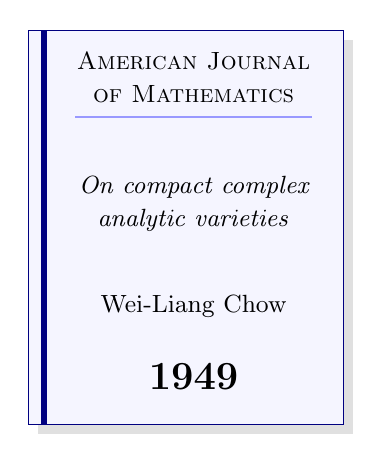
\begin{tikzpicture}
\fill[black!12] (.12,-.12) rectangle (4.12,4.88);
\filldraw[fill=blue!4,draw=blue!50!black] (0,0) rectangle (4.0,5.0);
\draw[blue!50!black,line width=2pt] (.2,0)--(.2,5.0);
\node[align=center,text width=3.4cm] at (2.1,4.4) {\small\textsc{American Journal of Mathematics}};
\draw[blue!40] (.6,3.9)--(3.6,3.9);
\node[align=center,text width=3.1cm] at (2.1,2.8) {\small\emph{On compact complex analytic varieties}};
\node[align=center] at (2.1,1.5) {\small Wei-Liang Chow};
\node at (2.1,.6) {\Large\textbf{1949}};
\end{tikzpicture}
\column{.56\textwidth}
\begin{itemize}
\setlength{\itemsep}{8pt}
\item Born in Shanghai in 1911. Bachelor's degree in Chicago, 1931; then Göttingen, then Leipzig.
\item Doctorate in Leipzig under \textbf{van der Waerden}.
\item Taught in Nanjing; his work was badly disrupted by the war. At the Institute for Advanced Study from 1947.
\item Professor at \textbf{Johns Hopkins}, 1948--1977, where he founded a school of algebraic geometry. Died in Baltimore in 1995.
\end{itemize}
\end{columns}
\par\medskip
His theorem, 1949: a compact analytic variety in projective space is algebraic.
\src{The picture is an illustration, not a facsimile. Sources: MacTutor, ``Wei-Liang Chow''; Wikipedia, ``Wei-Liang Chow''.}
\end{frame}

\begin{frame}{Where Chow's theorem sits in history}
\label{fr:chow-timeline}
\begin{center}
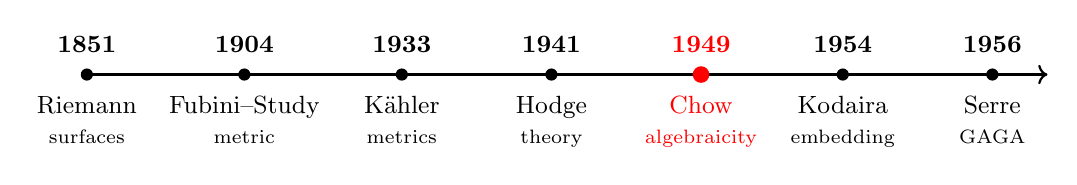
\begin{tikzpicture}[x=1.0cm]
\draw[thick,->] (0,0)--(12.2,0);
\foreach \x/\y/\t/\s in {
 0/1851/Riemann/surfaces,
 2.0/1904/Fubini--Study/metric,
 4.0/1933/Kähler/metrics,
 5.9/1941/Hodge/theory,
 9.6/1954/Kodaira/embedding,
 11.5/1956/Serre/GAGA}
{\fill (\x,0) circle (2.2pt);
 \node[above] at (\x,.15) {\small\textbf{\y}};
 \node[below,align=center] at (\x,-.15) {\small \t\\[-1pt]\scriptsize\s};}
\fill[red] (7.8,0) circle (3pt);
\node[above,red] at (7.8,.15) {\small\textbf{1949}};
\node[below,align=center,red] at (7.8,-.15) {\small Chow\\[-1pt]\scriptsize algebraicity};
\end{tikzpicture}
\end{center}
\par\bigskip
The timeline of lecture 23, with Chow added.
\par\medskip
\begin{itemize}
\setlength{\itemsep}{6pt}
\item \textbf{1949, Chow:} an analytic subvariety of \(\Pj^n\) is algebraic.
\item \textbf{1954, Kodaira:} a compact manifold with a positive line bundle embeds in \(\Pj^n\).
\item \textbf{Together:} such a manifold is a projective algebraic variety. Kodaira's theorem needs Chow's to reach algebra.
\item \textbf{1956, Serre (GAGA):} the same for sheaves and their cohomology.
\end{itemize}
\end{frame}

\begin{frame}{Why \(\operatorname{Pic}(\Pj^n)=\mathbb Z\)}
\label{fr:prov-od-0}
\textbf{1. Line bundles are cocycles.} A line bundle is given by transition functions \(g_{ij}\), holomorphic without zeros, with \(g_{ij}g_{jk}=g_{ik}\). So \(\operatorname{Pic}(X)=H^1(X,\cO^*)\).
\par\smallskip
\textbf{2. The exponential sequence} \(\ 0\to\mathbb Z\to\cO\xrightarrow{\,f\mapsto e^{2\pi if}\,}\cO^*\to0\ \) is exact: a function without zeros has a logarithm locally, and \(e^{2\pi if}=1\) exactly when \(f\) is an integer.
\par\smallskip
\textbf{3. The long exact sequence} contains
\[
H^1(X,\cO)\longrightarrow\operatorname{Pic}(X)\xrightarrow{\ c_1\ }H^2(X,\mathbb Z)\longrightarrow H^2(X,\cO).
\]
\textbf{4. On \(\Pj^n\) the outer groups vanish.} They are \(H^{0,1}\) and \(H^{0,2}\). By the CW decomposition, \(H^k(\Pj^n,\mathbb Z)\) is \(\mathbb Z\) for \(k\) even and \(0\) for \(k\) odd. So \(H^1=0\) gives \(H^{0,1}=0\); and \(H^2\) has rank \(1\), with \(h^{2,0}=h^{0,2}\), so \(H^{0,2}=0\). Hence
\[
\boxed{c_1:\operatorname{Pic}(\Pj^n)\ \xrightarrow{\ \cong\ }\ H^2(\Pj^n,\mathbb Z)=\mathbb Z .}
\]
\textbf{5.} \(\cO(1)\) goes to the generator. So every line bundle on \(\Pj^n\) is \(\cO(d)\), with \(d=c_1\).
\src{Huybrechts, \emph{Complex Geometry}, Exercise 3.2.11.}
\end{frame}


\begin{frame}{The bundles \(\cO(d)\)}
\label{fr:prov-od-1}
A point \(p\in\Pj^n\) is a line through the origin in \(\C^{n+1}\).
\par\medskip
\textbf{Definition.}
\begin{itemize}
\setlength{\itemsep}{10pt}
\item \(\cO(-1)\) is the tautological bundle: its fibre at \(p\) is the line \(p\) itself.
\item \(\cO(1):=\cO(-1)^\vee\), the dual bundle. Its fibre at \(p\) is the space of linear functionals on the line \(p\).
\item \(\cO(d):=\cO(1)^{\otimes d}\), the \(d\)-th tensor power.
\end{itemize}
\par\medskip
\textbf{Plan.} To show that the sections of \(\cO(d)\) are the homogeneous polynomials of degree \(d\):
\begin{enumerate}
\item the fibres are the homogeneous functions of degree \(d\) on the line (not yet polynomials);
\item a polynomial gives a section;
\item every section is a polynomial.
\end{enumerate}
\end{frame}

\begin{frame}{The fibre of \(\cO(d)\) at a point}
\label{fr:prov-od-2}
\textbf{Lemma.} The fibre \(\cO(d)_p\) is the space of homogeneous functions of degree \(d\) on the line \(p\).
\par\medskip
\textbf{Proof.}
\begin{enumerate}
\setlength{\itemsep}{6pt}
\item \(\cO(1)_p=\operatorname{Hom}(p,\C)\): the linear functionals on the line \(p\).
\item So \(\cO(d)_p=\operatorname{Hom}(p,\C)^{\otimes d}\cong\operatorname{Hom}(p^{\otimes d},\C)\). (True here because \(p\) has a basis.)
\item By the universal property of the tensor product, \(\operatorname{Hom}(p^{\otimes d},\C)\) is the set of multilinear maps \(L:p\times\cdots\times p\to\C\).
\item Such an \(L\) gives a function on \(p\), homogeneous of degree \(d\):
\[
P(x):=L(x,\ldots,x),\qquad P(\lambda x)=\lambda^dP(x).
\]
\item Conversely, \(p\) has dimension \(1\). Take a basis vector \(x\) and define \(L\) by \(L(x,\ldots,x):=P(x)\). This does not depend on \(x\): for \(x'=\lambda x\), both sides are multiplied by \(\lambda^d\).
\end{enumerate}
\end{frame}

\begin{frame}{A polynomial is a section}
\label{fr:prov-od-3}
\textbf{Exercise.} A nonzero homogeneous polynomial \(P\in\C[z_0,\ldots,z_n]_d\) is a nonzero section of \(\cO(d)\) on \(\Pj^n\).
\par\medskip
\begin{enumerate}
\setlength{\itemsep}{12pt}
\item \textbf{Define it fibre by fibre.} For \(p\in\Pj^n\), restrict \(P\) to the line \(p\). This is a homogeneous function of degree \(d\) on \(p\): an element of \(\cO(d)_p\) (lemma).
\item \textbf{It is holomorphic} (next slide).
\item \textbf{Where it vanishes.} The section is zero at \(p\) exactly when \(P\) is zero on the line \(p\). So
\[
\boxed{\text{its zero set is } \{P=0\}\subset\Pj^n .}
\]
\end{enumerate}
\src{Huybrechts, \emph{Complex Geometry}, Exercise 2.2.8. J.~M.~Lee, \emph{Introduction to Complex Manifolds}, Lemma 3.30 and Proposition 3.35.}
\end{frame}

\begin{frame}{Why that section is holomorphic}
\label{fr:prov-od-3b}
\textbf{A point of \(\Pj^n\) is a line.} The line \(p\) through the origin consists of all multiples of one nonzero vector \(z\): \(\ p=\{\lambda z:\ \lambda\in\C\}\), \(\ z=(z_0,\ldots,z_n)\).
\par\smallskip
\textbf{Look for the multiple whose \(i\)-th coordinate is \(1\).} The \(i\)-th coordinate of \(\lambda z\) is \(\lambda z_i\). On the chart \(z_i\ne0\) there is exactly one such multiple, \(\lambda=1/z_i\). Call it \(\sigma_i(p)\):
\[
\sigma_i(p)=\frac{z}{z_i}=\Bigl(\frac{z_0}{z_i},\ldots,1,\ldots,\frac{z_n}{z_i}\Bigr).
\]
\textbf{One number determines a function on the line.} A homogeneous function \(\varphi\) of degree \(d\) on \(p\) is determined by the number \(\varphi(\sigma_i(p))\), since \(\varphi(\lambda x)=\lambda^d\varphi(x)\).
\par\smallskip
\textbf{That number is a coordinate.} Let \(\varphi_0\) be the function with \(\varphi_0(\sigma_i(p))=1\): a basis of the fibre \(\cO(d)_p\). Then \(\ \varphi=\varphi(\sigma_i(p))\cdot\varphi_0\). So \(\varphi(\sigma_i(p))\) is the coordinate of \(\varphi\) in the fibre.
\par\smallskip
\textbf{For our section} the coordinate is \(\ P(\sigma_i(p))=P\bigl(z_0/z_i,\ldots,1,\ldots,z_n/z_i\bigr)\), a polynomial in the chart coordinates \(z_k/z_i\). So the section is holomorphic.
\end{frame}




\begin{frame}{Every section is a polynomial}
\label{fr:prov-od-4}
\textbf{Theorem.} The sections of \(\cO(d)\) are exactly the homogeneous polynomials of degree \(d\).
\par\medskip
\textbf{Proof.} It remains to show that a section \(s\in H^0(\Pj^n,\cO(d))\) is a polynomial.
\begin{enumerate}
\setlength{\itemsep}{6pt}
\item For each \(p\), \(s(p)\in\cO(d)_p\) is a homogeneous function \(f_p\) of degree \(d\) on the line \(p\) (lemma).
\item \textbf{Put them together.} For \(z\in\C^{n+1}\setminus\{0\}\) let \(p\) be the line through \(z\), and define
\[
f(z):=f_p(z).
\]
Then \(f\) is holomorphic on \(\C^{n+1}\setminus\{0\}\), and \(f(\lambda z)=\lambda^df(z)\).
\item \textbf{Hartogs' theorem:} \(f\) extends to a holomorphic function on \(\C^{n+1}\).
\item \textbf{Taylor series at \(0\):} \(f=\sum_jf_j\), with \(f_j\) homogeneous of degree \(j\). Then \(f(\lambda z)=\lambda^df(z)\) forces \(f=f_d\): a homogeneous polynomial of degree \(d\).
\end{enumerate}
\src{J.~M.~Lee, \emph{Introduction to Complex Manifolds}, Theorem 3.36.}
\end{frame}

\begin{frame}{A smooth hypersurface is \(\{F=0\}\)}
\label{fr:chow-3}
Let \(V\subset\Pj^n\) be a smooth closed complex hypersurface.
\par\smallskip
\textbf{1. Local equations.} Cover \(\Pj^n\) by open sets \(U_i\) on which \(V=\{g_i=0\}\), with \(g_i\) holomorphic and vanishing to first order along \(V\): in coordinates where \(V=\{z_1=0\}\), take \(g_i=z_1\).
\par\smallskip
\textbf{2. They differ by units.} On \(U_i\cap U_j\) both \(g_i\) and \(g_j\) vanish exactly on \(V\), to first order. So \(\ g_{ij}=g_i/g_j\ \) is holomorphic and has no zeros.
\par\smallskip
\textbf{3. A line bundle and a section.} The \(g_{ij}\) satisfy \(g_{ij}g_{jk}=g_{ik}\): they are the transition functions of a line bundle \(\cO(V)\). And \(g_i=g_{ij}\,g_j\) says that the \(g_i\) glue to one global section \(s_V\) of \(\cO(V)\), with zero set exactly \(V\).
\par\smallskip
\textbf{4. Use the previous slides.} \(\cO(V)=\cO(d)\) for some \(d\), and its section \(s_V\) is a homogeneous polynomial \(F\) of degree \(d\). So \(\ \boxed{V=\{F=0\}.}\)
\par\smallskip
\textbf{This proves Chow's theorem up to the higher codimension step} (next slide).
\end{frame}

\begin{frame}{Higher codimension (roughly)}
\label{fr:chow-4}
Let \(V\subset\Pj^n\) have dimension \(k<n-1\). It is not a hypersurface, so we make it one.
\par\medskip
\textbf{1. Project.} Choose a linear subspace \(\Pj^{n-k-2}\) not meeting \(V\), and project from it onto a complementary \(\Pj^{k+1}\). The image of \(V\) is a hypersurface in \(\Pj^{k+1}\) (not proved).
\par\medskip
\textbf{2. Apply the previous slide.} The image is \(\{F=0\}\) for a homogeneous polynomial \(F\) in \(x_0,\ldots,x_{k+1}\).
\par\medskip
\textbf{3. Pull back.} Read \(F\) as a polynomial \(\widetilde F\) in all the variables \(x_0,\ldots,x_n\). Then \(\widetilde F\) vanishes on \(V\).
\par\medskip
\textbf{4. Enough equations.} For each point \(q\notin V\), the subspace can be chosen so that \(q\) does not project into the image of \(V\). Then \(\widetilde F(q)\ne0\). So \(V\) is the common zero set of these \(\widetilde F\), one for each \(q\). Finitely many suffice.
\par\medskip
The projection of a smooth \(V\) can be singular, so the previous slide is needed for singular hypersurfaces too (not proved).
\end{frame}

\begin{frame}{Kawamata--Viehweg vanishing: the statement}
\label{fr:kv-statement}
Let \(X\) be a projective manifold of dimension \(n\), and \(L\) a holomorphic line bundle on \(X\).
\par\smallskip
\textbf{Definition.} \(L\) is \textbf{nef} if \(\int_Sc_1(L)\ge0\) for every curve \(S\subset X\).
\par\smallskip
Equivalently: \(c_1(L)\) lies in the closure of the Kähler cone.
\par\medskip
\textbf{Definition.} \(L\) is \textbf{big} if \(\ \limsup_{k}\,\dim H^0(X,L^k)/k^n>0\).
\par\smallskip
That is: \(\dim H^0(X,L^N)\ge b\cdot N^n\) for some \(b>0\) and infinitely many \(N\). So the number of independent sections of \(L^N\) on \(X\) grows like \(N^n\), where \(n=\dim X\).
\par\medskip
\textbf{Theorem (Kawamata--Viehweg).} If \(L\) is nef and big, then
\[
\boxed{H^i(X,K_X\otimes L)=0\qquad\text{for all } i>0 .}
\]
\textbf{Compare with Kodaira vanishing:} the same conclusion, for \(L\) positive. Positive implies nef and big, but not conversely. So ``positive'' is weakened to ``nef and big''.
\src{M.~Verbitsky, \emph{Hodge theory}, lecture 24 (2025), slides 13 and 14.}
\end{frame}

\begin{frame}{Yujiro Kawamata and Eckart Viehweg}
\label{fr:kv-people}
\begin{columns}[t]
\column{.48\textwidth}
\centering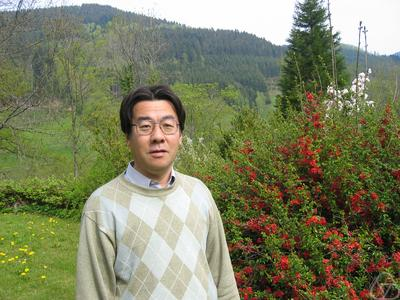
\includegraphics[width=\linewidth,height=2.5cm,keepaspectratio]{../assets/Yujiro_Kawamata.png}
\par\smallskip\textbf{Yujiro Kawamata} (born 1952)
\par\smallskip
\raggedright\small
\begin{itemize}
\item University of Tokyo; student of Shigeru Iitaka.
\item Minimal model program, 1980s.
\item Japan Academy Prize, 1990.
\end{itemize}
\column{.48\textwidth}
\centering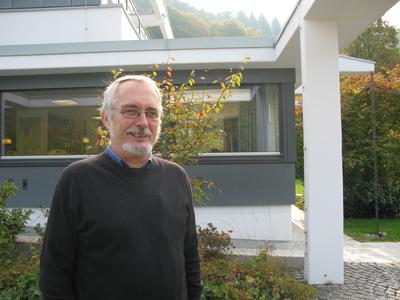
\includegraphics[width=\linewidth,height=2.5cm,keepaspectratio]{../assets/Eckart_Viehweg.png}
\par\smallskip\textbf{Eckart Viehweg} (1948--2010)
\par\smallskip
\raggedright\small
\begin{itemize}
\item Born in Zwickau; professor in Essen from 1984.
\item Worked with Hélène Esnault.
\item Leibniz Prize, 2003, with Esnault.
\end{itemize}
\end{columns}
\par\medskip
\centering Two independent papers in 1982: positivity can be weakened to \textbf{nef and big}.
\src{Photos: Renate Schmid / MFO, Oberwolfach 2004 and 2009, CC BY-SA 2.0 DE. Papers: Kawamata, Math. Ann. 261 (1982), 43--46; Viehweg, J. reine angew. Math. 335 (1982), 1--8.}
\end{frame}

\begin{frame}{Where Kawamata--Viehweg sits in history}
\label{fr:kv-timeline}
\begin{center}
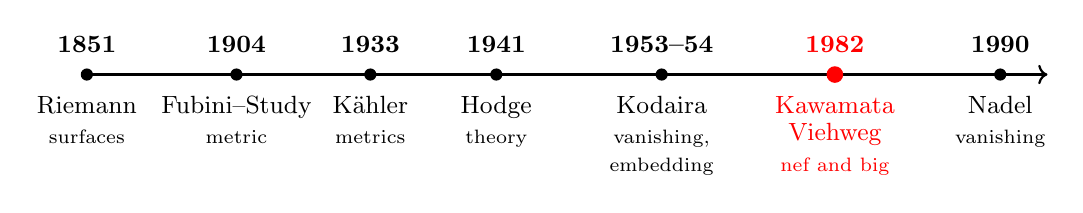
\begin{tikzpicture}[x=1.0cm]
\draw[thick,->] (0,0)--(12.2,0);
\foreach \x/\y/\t/\s in {
 0/1851/Riemann/surfaces,
 1.9/1904/Fubini--Study/metric,
 3.6/1933/Kähler/metrics,
 5.2/1941/Hodge/theory,
 7.3/1953--54/Kodaira/{vanishing{,}\\[-2pt]\scriptsize embedding},
 11.6/1990/Nadel/vanishing}
{\fill (\x,0) circle (2.2pt);
 \node[above] at (\x,.15) {\small\textbf{\y}};
 \node[below,align=center] at (\x,-.15) {\small \t\\[-1pt]\scriptsize\s};}
\fill[red] (9.5,0) circle (3pt);
\node[above,red] at (9.5,.15) {\small\textbf{1982}};
\node[below,align=center,red] at (9.5,-.15) {\small Kawamata\\[-2pt]\small Viehweg\\[-1pt]\scriptsize nef and big};
\end{tikzpicture}
\end{center}
\par\medskip
This is the timeline of lecture 23, with one new point.
\par\smallskip
\begin{itemize}
\setlength{\itemsep}{6pt}
\item \textbf{1953, Kodaira:} vanishing for a \emph{positive} line bundle.
\item \textbf{1954, Kodaira:} embedding, one year later, proved with the vanishing theorem.
\item \textbf{1982, Kawamata and Viehweg:} vanishing for a \emph{nef and big} line bundle.
\item \textbf{1990, Nadel:} vanishing with a multiplier ideal.
\end{itemize}
\par\medskip
We prove the 1982 theorem with the 1990 tool: an older theorem through a newer one.
\end{frame}

\begin{frame}{Kawamata--Viehweg: the proof is one lemma and Nadel}
\label{fr:kv-proof-1}
\textbf{Lemma.} Let \(L\) be a nef and big line bundle on a projective manifold \(X\). Then \(L\) has a singular metric \(h\) with
\[
\boxed{i\Theta_h\ge\varepsilon\omega\ \ (\varepsilon>0)\qquad\text{and}\qquad\cI(h)=\cO_X .}
\]
\textbf{The lemma gives the theorem.} By Nadel, for \(i>0\),
\[
H^i(X,K_X\otimes L\otimes\cI(h))=0,\qquad\text{and}\quad\cI(h)=\cO_X .
\]
So \(H^i(X,K_X\otimes L)=0\).
\par\bigskip
\textbf{Compare with the embedding proof.} There we wanted \(\cI(h)\) to be \(\mathfrak m_x\), \(\mathfrak m_x\cap\mathfrak m_y\), \(\mathfrak m_x^2\): poles strong enough to impose conditions. Here we want the opposite: a singular metric whose poles are so mild that the ideal does not see them.
\src{M.~Verbitsky, \emph{Hodge theory}, lecture 24 (2025), slide 14.}
\end{frame}

\begin{frame}{Reminder: ample line bundles}
\label{fr:kv-ample}
\textbf{Definition.} \(L\) is \textbf{very ample} if its global sections give an embedding \(\Phi_L:X\hookrightarrow\Pj(H^0(X,L)^*)\). That is: no common zero, they separate points, they separate tangents (slide \hyperlink{fr:goal-sections}{\pageref{fr:goal-sections}}).
\par\medskip
\textbf{Definition.} \(L\) is \textbf{ample} if \(L^N\) is very ample for some \(N>0\).
\par\medskip
\textbf{Theorem (Kodaira).} \(\ \boxed{L \text{ is ample}\iff L \text{ is positive}}\ \): it has a smooth metric with \(i\Theta_h>0\).
\begin{itemize}
\setlength{\itemsep}{5pt}
\item \(\Leftarrow\) is the embedding theorem we just proved (slide \hyperlink{fr:conclusion}{\pageref{fr:conclusion}}).
\item \(\Rightarrow\): if \(L^N\) is very ample, then \(L^N=\Phi^*\cO(1)\). Pull back the Fubini--Study metric of \(\cO(1)\): its curvature is positive on \(\Pj^M\), hence on the submanifold \(X\). The \(N\)-th root is a metric on \(L\) with positive curvature.
\end{itemize}
\par\medskip
\textbf{So three ways to say the same thing:} \(L\) is ample; \(L\) is positive; \(c_1(L)\) is the class of a Kähler form.
\src{M.~Verbitsky, \emph{Hodge theory}, lecture 24 (2025), slide 12.}
\end{frame}

\begin{frame}{Reminder: divisors}
\label{fr:kv-divisors}
\textbf{Divisor.} A finite formal sum \(D=\sum a_iV_i\), with \(V_i\subset X\) hypersurfaces and \(a_i\in\mathbb Z\).
\par\smallskip
It is \textbf{effective} if all \(a_i\ge0\).
\par\bigskip
\textbf{From a divisor to a line bundle.} In the proof of Chow (slide \hyperlink{fr:chow-3}{\pageref{fr:chow-3}}) a hypersurface \(V\) gave a line bundle \(\cO(V)\) with a section vanishing exactly on \(V\). For a divisor,
\[
\cO(D)=\bigotimes_i\cO(V_i)^{\otimes a_i} .
\]
\textbf{From a section to a divisor.} If a line bundle \(L\) has a holomorphic section \(s\ne0\), the zeros of \(s\), counted with multiplicity, form an effective divisor \(D\), and \(L=\cO(D)\).
\par\bigskip
\textbf{Ample divisor:} a divisor \(Y\) with \(\cO(Y)\) ample (previous slide). Example: a hyperplane section of \(X\subset\Pj^M\).
\end{frame}


\begin{frame}{Ample and nef in the Kähler cone}
\label{fr:kv-cone}
\begin{columns}[T]
\column{.60\textwidth}
\textbf{The Kähler cone:} the classes in \(H^{1,1}(X,\mathbb R)\) of Kähler forms. It is an \textbf{open convex cone}: sums and positive multiples of Kähler forms are Kähler, and a small change of a positive form stays positive.
\par\smallskip
\textbf{Ample} \(=\) positive (Kodaira):\\ \(c_1(L)\) is \emph{inside} the cone.
\par\smallskip
\textbf{Nef:} \(c_1(L)\) is in the \emph{closure} of the cone, inside or on the boundary. It is a limit of Kähler classes.
\column{.36\textwidth}
\centering
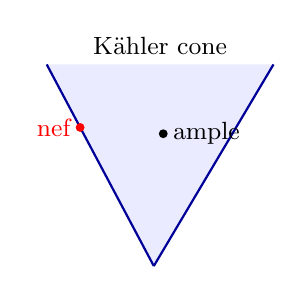
\begin{tikzpicture}[scale=.8]
\fill[blue!8] (0,0)--(-1.7,3.2)--(1.9,3.2)--cycle;
\draw[thick,blue!60!black] (0,0)--(-1.7,3.2);
\draw[thick,blue!60!black] (0,0)--(1.9,3.2);
\fill (0.15,2.1) circle (2pt) node[right] {\small ample};
\fill[red] (-1.17,2.2) circle (2pt) node[left,red] {\small nef};
\node at (0.1,3.5) {\small Kähler cone};
\end{tikzpicture}
\end{columns}
\par\smallskip
\textbf{Why this is the definition with curves.} For a Kähler form, \(\int_S\omega>0\) on every curve \(S\). In the limit, \(\int_Sc_1(L)\ge0\). The converse is a theorem (Demailly--Paun; not proved).
\src{M.~Verbitsky, \emph{Hodge theory}, lecture 24 (2025), slide 13.}
\end{frame}

\begin{frame}{Nef plus ample is ample}
\label{fr:kv-nef-ample}
\textbf{An open cone absorbs its boundary.} Let \(\alpha\) be in the closure of the Kähler cone and \(\omega\) inside it. Then \(\alpha+\omega\) is inside.
\par\medskip
\textbf{Why.} \(\alpha\) is a limit of Kähler classes \(\alpha_k\). Write
\[
\alpha+\omega=\alpha_k+\bigl(\omega-(\alpha_k-\alpha)\bigr).
\]
For \(k\) large, \(\alpha_k-\alpha\) is small, so \(\omega-(\alpha_k-\alpha)\) is still inside (the cone is open). A sum of two classes inside the cone is inside (the cone is convex).
\par\bigskip
\textbf{For line bundles.} Let \(L\) be nef and \(Y\) an ample divisor. For every \(N\ge0\),
\[
c_1\bigl(L^N\otimes\cO(Y)\bigr)=N\,c_1(L)+c_1(\cO(Y)),
\]
closure plus inside. So this class is inside the cone, and
\[
\boxed{L^N\otimes\cO(Y)\ \text{ is ample, for every } N\ge0 .}
\]
\src{M.~Verbitsky, \emph{Hodge theory}, lecture 24 (2025), slide 16, step 1.}
\end{frame}


\begin{frame}{Proof of the lemma: three ingredients}
\label{fr:kv-proof-2}
\begin{enumerate}
\setlength{\itemsep}{9pt}
\item \textbf{Nef plus ample is ample} (slide \hyperlink{fr:kv-nef-ample}{\pageref{fr:kv-nef-ample}}): for \(L\) nef and \(Y\) ample, \(L^N\otimes\cO(Y)\) is ample for every \(N\ge0\).
\item \textbf{Sections grow at most like \(N^{\dim}\).} For any line bundle on a projective manifold of dimension \(m\), \(\ \dim H^0(L^N)\le R\cdot N^m\). \textbf{Big} means: \(\dim H^0(X,L^N)\ge b\cdot N^n\) for some \(b>0\) and infinitely many \(N\).
\item \textbf{A mild pole along a divisor is invisible.} Let \(H\) be a holomorphic function with zero divisor \(D\). The metric \(e^{-2\alpha\log|H|}\) has trivial multiplier ideal when \(\alpha>0\) is small enough: \(|H|^{-2\alpha}\) is locally integrable.
\end{enumerate}
\src{M.~Verbitsky, \emph{Hodge theory}, lecture 24 (2025), slides 4, 15 and 16.}
\end{frame}

\begin{frame}{Why sections grow at most like \(N^{\dim}\)}
\label{fr:kv-growth}
\textcolor{red}{\textbf{Claim.}} For a projective manifold \(M\) of dimension \(m\) and any line bundle \(L\) on it, \(\ P(N):=\dim H^0(M,L^N)\le R\cdot N^m\).
\par\smallskip
\textbf{Model:} on \(\Pj^m\), \(\dim H^0(\cO(N))=\binom{N+m}{m}\approx N^m/m!\).
\par\smallskip
\textbf{Proof,} by induction on \(m\).
\begin{enumerate}
\setlength{\itemsep}{2pt}
\item \(m=0\): \(M\) is finitely many points, and \(P(N)\) is their number.
\item We may assume \(L\) has a section \(s\ne0\) (otherwise pass to a power of \(L\) that has one). Its zero divisor \(D\) has dimension \(m-1\).
\item Multiplying by \(s\) gives \(\ 0\to L^{N-1}\xrightarrow{\,\cdot s\,}L^N\to L^N|_D\to0\). On sections, by induction: \(\ P(N)-P(N-1)\le\dim H^0(D,L^N|_D)\le R'\cdot N^{m-1}\).
\item Add up: \(\ P(N)\le P(0)+R'\cdot(1^{m-1}+\cdots+N^{m-1})\le R\cdot N^m\).
\end{enumerate}
\textbf{For us:} \(Y\) has dimension \(n-1\), so \(\ \boxed{\dim H^0(Y,L^N|_Y)\le R\cdot N^{n-1}.}\)
\src{M.~Verbitsky, \emph{Hodge theory}, lecture 24 (2025), slide 15. \(D\) may be singular: the induction is really over varieties (not proved).}
\end{frame}


\begin{frame}{Proof of the lemma: a section of \(L^d\otimes\cO(-Y)\)}
\label{fr:kv-proof-3}
Fix \(X\subset\Pj^M\) and let \(Y\) be a smooth hyperplane section: an ample divisor. Restrict to \(Y\):
\[
0\longrightarrow L^N\otimes\cO(-Y)\longrightarrow L^N\longrightarrow L^N|_Y\longrightarrow0 .
\]
On global sections:
\vspace{-3pt}
\[
0\longrightarrow H^0(X,L^N\otimes\cO(-Y))\longrightarrow H^0(X,L^N)\longrightarrow H^0(Y,L^N|_Y).
\]
\begin{itemize}
\setlength{\itemsep}{2pt}
\item \(\dim H^0(X,L^N)\ge b\cdot N^n\) for some \(b>0\) and infinitely many \(N\), because \(L\) is big.
\item \(\dim H^0(Y,L^N|_Y)\le R\cdot N^{n-1}\), because \(\dim Y=n-1\) (previous slide).
\end{itemize}
\(N^n\) grows faster than \(N^{n-1}\). So for some large \(N\), which we call \(d\): \(\ \dim H^0(X,L^d)>\dim H^0(Y,L^d|_Y)\), and the restriction map has a kernel.
\[
\boxed{L^d\otimes\cO(-Y)\ \text{has a nonzero section. Let } D \text{ be its zero divisor.}}
\]
\src{M.~Verbitsky, \emph{Hodge theory}, lecture 24 (2025), slide 16, step 2.}
\end{frame}

\begin{frame}{Proof of the lemma: the metric}
\label{fr:kv-proof-4}
For \(N\ge d\), split \(L^N\) into an ample part and the divisor:
\[
L^N=\bigl(L^{N-d}\otimes\cO(Y)\bigr)\otimes\cO(D).
\]
\begin{itemize}
\setlength{\itemsep}{2pt}
\item \(L^{N-d}\otimes\cO(Y)\) is ample (slide \hyperlink{fr:kv-nef-ample}{\pageref{fr:kv-nef-ample}}): it has a smooth metric \(h_1\) with curvature \(\omega>0\).
\item \(\cO(D)\) has a singular metric \(h_0\) with curvature the current \([D]\ge0\): locally \(h_0=e^{-2\log|H|}\), with \(H\) an equation of \(D\) (\textcolor{red}{Poincaré--Lelong}).
\end{itemize}
So \(h_0h_1\) on \(L^N\) has curvature \(\omega+[D]\). Its \(N\)-th root is a metric \(h\) on \(L\):
\[
\boxed{i\Theta_h=\frac1N\,\omega+\frac1N\,[D]\ \ge\ \frac1N\,\omega .}
\]
\textbf{Multiplier ideal:} locally \(h=(\text{smooth})\cdot e^{-\frac2N\log|H|}\), a pole with coefficient \(1/N\): invisible for \(N\) large (slide \hyperlink{fr:kv-proof-2}{\pageref{fr:kv-proof-2}}). So \(\cI(h)=\cO_X\).
\src{M.~Verbitsky, \emph{Hodge theory}, lecture 24 (2025), slide 16, step 3.}
\end{frame}

\end{document}
